%\documentclass[a4paper,11pt]{article}
\documentclass[a4paper,11pt,twoside]{article}
\usepackage{latexsym}
\usepackage[polish]{babel}
\usepackage{amsmath}
\usepackage{physics}
\usepackage[utf8]{inputenc}
\usepackage[T1]{fontenc}
\usepackage[usenames,dvipsnames]{color}
\usepackage[table]{xcolor}
\usepackage[pdftex]{graphicx}
\usepackage{fancyhdr}
\usepackage{listings}
\usepackage{hyperref}
\usepackage[margin=2.5cm]{geometry}
\usepackage{rotating}
\usepackage{url}
\pagestyle{fancy}
\fancypagestyle{firststyle}
{
   \fancyhf{}
   \renewcommand{\headrulewidth}{0pt}
   \fancyfoot[C]{Czerwiec 2015}
}
\date{}
\title{\Huge Symulacje komputerowe dynamiki płynów \\
 \Large Raport z implementacji modelu LBM-MRT}
\definecolor{LightGray}{RGB}{230, 230, 230}
\definecolor{DarkGreen}{RGB}{0, 180, 0}
\definecolor{DarkRed}{RGB}{180, 0, 0}
\definecolor{DarkBlue}{RGB}{0, 0, 100}
\author{Jakub Poła}
\begin{document}

\maketitle
\thispagestyle{firststyle}
\newpage
\tableofcontents
\newpage

\section{Wstęp}
Celem projektu było zaimplementowanie algortymu gazu sieciowego Boltzmanna (LBM), operatora kolizji w przybliżeniu Bhatnagar–Gross–Krook (BGK) \cite{BGK} oraz w przybliżeniu MRT (Multiple Relaxation Time). Projekt zrealizowano w technologii C++ wykorzystując pakiet openFrameworks \cite{OpenFrameworks} do wizualizacji symulacji.

\section{Model gazu sieciowego Boltzmanna}
Rozważmy dwuwymiarowy układ zbudowany z $N$ punktów materialnych, każdy o masie $m$, oddziałujących tylko ze sobą. Chcąc poznać ewolucję tego układu należy rozwiązać dla niego $4N$ równań Newtona:
\begin{eqnarray}
\frac{dx_i}{dt} = \frac{p_i}{m} \\
\label{NewtEq1}
\frac{dp_i}{dt} = F_i
\label{NewtEq2}
\end{eqnarray}

gdzie $x_i$ jest wektorem położenia punktu $i$, $p_i$ pędem punktu $i$, $F_i$ wypadkową siłą wzajemnego oddziaływania $i$-tego punktu z pozostałymi, $t$ czasem. W przypadku badania 1 mola gazu doskonałego, w którym znajduje się około $6.02 \times 10^{23}$ cząstek, rozwiązanie takiego układu równań staje się niezwykle uciążliwe. Z tego powodu stworzone zostało odmienne podejście do analizy tego typu układów. Wprowadzona została wielkość $f(x, p, t)$ zwana gęstością prawdopodobieństwa lub funkcją rozkładu o następującej własności:
\begin{equation}
\Delta n = f(x, p, t)\Delta x \Delta p
\label{dist_particles}
\end{equation}
$\Delta n$, jest prawdopodobną liczbą cząstek w położeniu $x$ o pędzie $p$. Ewolucję powyższego układu rozważanego w podejściu statystycznym opisuje równanie Boltzmanna:
\begin{equation}
\frac{\partial f}{\partial t} + \nabla \cdot f = \Omega
\label{Boltzmann_eq}
\end{equation}

Wielkość po prawej stronie równania \ref{Boltzmann_eq} modeluje oddziaływania międzycząsteczkowe i jest zwana całką lub operatorem kolizji.

\section{Operator kolizji}
Operator kolizji w równaniu Boltzmanna jest wyrażeniem całkowym. Dla układu dwóch cząstek traktowanych, jako sferyczne ciała sztywne oraz przy założeniu tylko bliskich oddziaływań operator zderzenia może być zapisany w następujący sposób:
\begin{equation}
\Omega(f) = \int (f'_{12} - f_{12})(p_1 - p_2) \sigma(p_1 - p_2, \omega ) d\omega dp
\label{collision_eq}
\end{equation}
, gdzie $\omega$ jest kątem bryłowym, w który cząstka została rozproszona, $f_{12}$ jest dwucząstkową funkcją rozkładu przed zderzeniem, $f'_{12}$ dwucząstkową funkcją rozkładu po zderzeniu.
\subsection{Aproksymacja BGK}
Aproksymacja BGK zakłada, że układ dąży do osiągnięcia równowagi termodynamicznej $f \rightarrow f^{eq}$, określoną np. przez rozkład Maxwella. Każde zderzenie powoduje odchylenie od stanu równowagi po czym układ wraca do niego w czasie $\tau$. Całka kolizji w przybliżeniu BGK wyrażona jest następującym równaniem:
\begin{equation}
\Omega(f) = \frac{f^{eq}-f}{\tau}
\label{BGK_eq}
\end{equation}


\subsection{Aproksymacja MRT}
Aproksymacja operatora kolizji w przybliżeniu MRT może być traktowana jako uogólnienie aproksymacji BGK, która często określana jest mianem 'Single Relaxation Time' (SRT). Nazwa pochodzi od faktu istnienia czasu relaksacji $\tau$.

W ogólności liniową aproksymację operatora kolizji możemy przedstawić jako:
\begin{equation}
\Omega(f) = -S(f- f^{eq})
\label{relaxation_eq}
\end{equation}
$S$ jest macierzą relaksacji, której rozmiar zależy od przyjętego modelu. W przybliżeniu BGK $S=\frac{1}{\tau}I$.
Przybliżenie MRT polega na przejściu z przestrzeni dystrybucji do przestrzeni odpowienich momentów tej funkcji, a następnie relaksacji tych momentów do stanu równowagi. Macierz transformacji z przestrzeni dystrybucji do przestrzeni momentów dla modelu D2Q9 wygląda następująco:

\begin{equation}
M = 
\begin{bmatrix}
			1 & 1 & 1 & 1 & 1 & 1 & 1 & 1 & 1	\\
			-4 & -1 & -1 & -1 & -1 & 2 & 2 & 2 & 2	\\
			4 & -2 &-2 & -2 & -2 & 1 & 1 & 1 & 1	\\
			0 & 1 & 0 & -1 & 0 & 1 & -1 & -1 & 1	\\
			0 & -2 & 0 & 2 & 0 & 1 & -1 & -1 & 1	\\
			0 &  0 & 1 & 0 & -1 & 1 & 1 &-1 & -1	\\
            0 & 0 & -2 & 0 & 2 & 1 & 1 & -1 & -1	\\
			0 & 1 & -1 & 1 & -1 & 0 & 0 & 0 & 0	\\
			0 & 0 & 0 & 0 & 0 & 1 & -1 & 1 & -1
\end{bmatrix}
\end{equation}
            
Wartości współczynników macierzy wynikają z postaci równań wyrażających poszczególne momenty funkcji rozkładu. P. Lallemand \cite{MRT} proponuje użycie następujących momentów $\ket{\rho} $ gęstość,  $\ket{\epsilon}$ energia, $\ket{\varepsilon}$ funkcja kwadratu energii, $\ket{j_x}$, $\ket{j_y}$ pęd odpowiednio w kierunku $x$ oraz $y$. $\ket{q_x}$, $\ket{q_y}$ strumień energii w kierunku $x$ i $y$, $\ket{p_{xx}}$, $\ket{p_{xy}}$ diagonalna i pozadiagonalna składowa tęsora naprężeń.
\begin{eqnarray}
&\ket{\rho} = (1, 1, 1, 1, 1, 1, 1, 1, 1)^T		\\
&\ket{\epsilon} = (-4, -1 , -1 , -1 , -1 , 2 , 2 , 2 , 2)^T\\
&\ket{\varepsilon} =(4 , -2 ,-2 , -2 , -2 , 1 , 1 , 1 , 1)^T 	\\
&\ket{j_x} = (0 , 1 , 0 , -1 , 0 , 1 , -1 , -1 , 1)^T \\
&\ket{j_y} = (0 , -2 , 0 , 2 , 0 , 1 , -1 , -1 , 1)^T\\
&\ket{q_x} = (0 ,  0 , 1 , 0 , -1 , 1 , 1 ,-1 , -1)^T \\
&\ket{q_y} = (0 , 0 , -2 , 0 , 2 , 1 , 1 , -1 , -1)^T \\ 
&\ket{p_{xx}} =(0 , 1 , -1 , 1 , -1 , 0 , 0 , 0 , 0)^T \\ 
&\ket{p_{xy}} = (0 , 0 , 0 , 0 , 0 , 1 , -1 , 1 , -1)^T
\end{eqnarray}

Relaksacja każdego z momentów wygląda tak samo jak relaksacja funkcji dystrybucji \ref{relaxation_eq}
\begin{equation}
\Omega(m_i) = - S_i(m_i - m^{eq})
\label{moment_relaxation_eq}
\end{equation}
$m_i$ i-ty moment funkcji rozkładu, $S_i$ czas relaksacji i-tego momentu. Stąd również pochodzi nazwa modelu. Do dyspozycji mamy 9 momentów oraz 9 odpowiadających im czasów relaksacji. Traktując momenty jako wektor $\ket{m} = (\rho, \epsilon, \varepsilon, j_x, q_x, j_y, q_y, p_{xx}, p_{xy})^T$ przejście pomiędzy przestrzeniami dystrybucji $\ket{f}$ i momentów  $\ket{m}$ możemy zapisać jako
\begin{eqnarray}
\ket{m} = M\ket{f} \\
\label{tr_f_m}
\ket{f} = M^{-1}\ket{m}
\label{tr_m_f}
\end{eqnarray}

Wartości równowagowe momentów wyznaczamy z równań:

\begin{eqnarray}
&m^{eq}_0 = \rho^{eq} = \rho \\
&m^{eq}_1 = \epsilon^{eq} = -2\rho + 3(j^2_x + j^2_y) \\
&m^{eq}_2 = \varepsilon^{eq} = \rho - 3(j^2_x + j^2_y)  \\
&m^{eq}_3 = j^{eq}_x\\ 
&m^{eq}_4 = q^{eq}_x = -j_x    \\ 
&m^{eq}_5 = j^{eq}_y = j_y  \\
&m^{eq}_6 = q^{eq}_y = -j_y      \\
&m^{eq}_7 = p^{eq}_xx = (j^2_x - j^2_y)  \\
&m^{eq}_8 = p^{eq}_xy = j_xj_y
\label{moment_equilibria}
\end{eqnarray}

gdzie $j_x = \rho u_x$, $j_y = \rho u_y$.

\section{Warunki brzegowe}
W modelu użyto warunków brzegowych typu no-slip.

\subsection{Warunki początkowe}
System inicjalizowany jest wartościami równowagowymi dystrybucji. Przepływ płynu wymuszany jest przez akcelerację odpowiednich elementów płynu zgodnie z równaniem (47) podanym przez M.Sukopa \cite{sukop}

\section{Wyniki}
Zastosowanie modelu MRT do symulacji przepływu płynu metodą LBM pozwala na badanie zjawisk przy znacznie wyższych liczbach Reynoldsa niż przy zastosowaniu modelu LBM-BGK. Test pozwoliły na osiągnięcie wartości $Re>10000$. Na rysunku \ref{MRT1} przedstawiona jest symulacja układu powszechnie znana jako cavity dla $Re=6000$. 
\begin{figure}[h]
\begin{center}
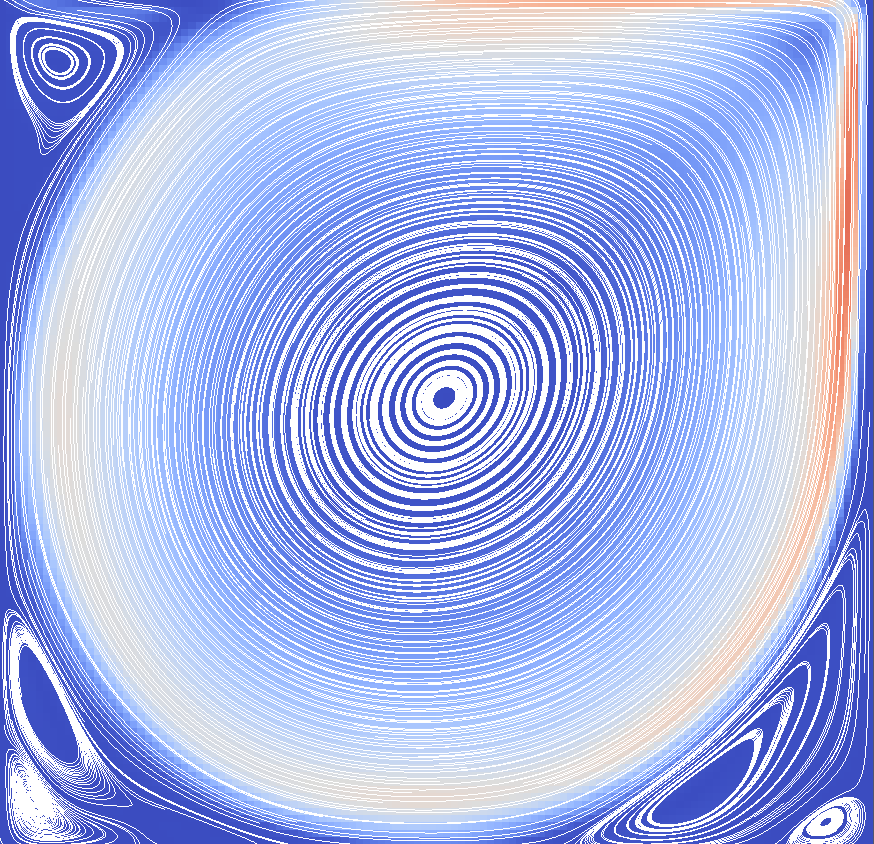
\includegraphics[width=0.75\linewidth]{images/6000.png}
\caption{Cavity Re=6000.}
\label{MRT1}
\end{center}
\end{figure}

\section{Kod programu}
Kod źródłowy zaimplementowaego modelu można pobrać z repozytoriun github: \url{https://github.com/jpola/LBM_CSCFD}. Projekt skonfigurowany jest za pomocą systemu CMAKE. Wymaga zainstalowania OpenFrameworks w wariancie CMake \url{https://github.com/ofnode/of} oraz rozszeżeń ofxGui i ofxColorMap.

\newpage
\bibliography{raport_bib}
\bibliographystyle{plain}
\end{document}